%Dokumentklasse
\documentclass[a4paper,12pt]{scrreprt}
\usepackage[left= 0.5cm,right = 0.5cm, bottom = 0 cm]{geometry}
%\usepackage[onehalfspacing]{setspace}
% ============= Packages =============

% Dokumentinformationen
\usepackage[
	pdftitle={Website-Penetration Testing},
	pdfsubject={},
	pdfauthor={Euer Name},
	pdfkeywords={},	
	%Links nicht einrahmen
	hidelinks
]{hyperref}


% Standard Packages
\usepackage[utf8]{inputenc}
%\usepackage[skip=0.333\baselineskip]{caption}
\usepackage{booktabs,tabularx,ragged2e}
\usepackage{graphicx, subfig}
\graphicspath{{img/}}
\usepackage{multirow}
\usepackage{ltablex}
\usepackage[ngerman]{babel}
\usepackage[T1]{fontenc}
\usepackage{fancyhdr}
\usepackage{lmodern}
\usepackage[export]{adjustbox}
\usepackage{setspace}
\usepackage{float}
\usepackage{multicol}
\usepackage{blindtext}
\usepackage[table]{xcolor}
\usepackage{tikz}
\usepackage{textpos}
\usepackage{afterpage}
\usepackage[nohyperlinks, printonlyused]{acronym}






% zusätzliche Schriftzeichen der American Mathematical Society
\usepackage{amsfonts}
\usepackage{amsmath}

%nicht einrücken nach Absatz
%\setlength{\parindent}{0pt}


% ============= Kopf- und Fußzeile =============
\pagestyle{fancy}
%
\lhead{}
\chead{}
\rhead{\slshape \leftmark}
%%
\lfoot{}
\cfoot{\thepage}
\rfoot{}
%%
\renewcommand{\headrulewidth}{0.4pt}
\renewcommand{\footrulewidth}{0pt}

% ============= Package Einstellungen & Sonstiges ============= 
%Besondere Trennungen
\hyphenation{De-zi-mal-tren-nung}


% ============= Dokumentbeginn =============

\begin{document}
%Seiten ohne Kopf- und Fußzeile sowie Seitenzahl
\pagestyle{empty}

\begin{center}
\begin{tabular}{p{\textwidth}}



\includegraphics[scale=0.5, right]{img/dhbw-logo.png}


\\

\begin{center}
\LARGE{\textsc{
Ethical Hacking:\\
Website-Penetration Testing \\
}}
\end{center}

\\


\begin{center}\large
    { im Studiengang}
\end{center}

\\

\begin{center}\large
    { Informatik Cybersecurity}
\end{center}

\begin{center}
an der dualen Hochschule Baden-Württemberg Mannheim
\end{center}


\begin{center}
von
\end{center}


\begin{center}
    \begin{tabular}{lll}
    \textbf{Name, Vorname:} & & Hartinger, Steven\\
    \textbf{Abgabedatum:} & & 01.09.2022\\
    \end{tabular}
    \end{center}

\\

\\

\begin{center}
\begin{tabular}{lll}
\textbf{Bearbeitungszeitraum:} & & 27.06.2022 - 01.09.2022\\
\textbf{Matrikelnummer, Kurs:} & & 7146735, TINF20CS1\\
\textbf{Ausbildungsunternehmen} & & MLP Finanzberatung SE\\
\textbf{Betrieblicher Betreuer:} & & Sebastian Damm\\

\\
\\


\end{tabular}
\end{center}

\end{tabular}
\end{center}

%Inhaltsverzeichnis
\tableofcontents

\chapter{Executive Summary}
\section*{Synopsis}
\hfill\break

As part of the lecture ''Offensive Security'' by Dr. Prof. Bauer the students of the TINF20CS1 performed a review on a Raspberry Pi handed by our lecturer. The objective of this task is to prepare a report on penetration testing for a Raspberry Pi B3+. The Raspberry Pi B3+ is powered by a 64-bit quad-core ARM Cortex-A53 CPU operating at 1.4GHz and has 1GB of LPDDR2 RAM. Its 40-pin GPIO header allows users to connect a diverse range of sensors and actuators, making it an excellent tool for development and learning. The device provided for this assignment comes with a 16GB microSD card, a 5V 2.5A power supply connected to a Micro-USB Cable, and a case. Our aim is to assess the security of the \ac{DUT}, including its OS and services, without prior knowledge of the specifics.
\section*{Scope}
\hfill \break

Our assessment included:
\begin{itemize}
    \item Validation of the given Raspberry Pi without exact requirements. 
    \item Provide countermeasures for vulnerablities of the system.
\end{itemize}

The threats included:
\begin{itemize}
    \item Network Eavesdrop - The attacker is on a wireless communication channel or somewhere else on the network
    \item Network Attack - The attacker is on a wireless communication channel or somewhere else on the network
    \item Physical Access - The attacker has physical access to the device
    \item Malicious Code - Malicious code loaded onto the Raspberry Pi
\end{itemize}

Testing was performed on:
\begin{itemize}
    \item Raspberry Pi 3
\end{itemize}

\section*{Limitations}
\section*{}

For this assessment we are not having any limitation besides a time limit.
\section*{Key Findings}
\hfill\break

This penetration test report revealed a significant number of critical findings that require immediate action to prevent potential security breaches. The test identified a total of 22 findings, including unauthorized access to the Device Under Test (DUT) and several misconfigurations that could be exploited by attackers. \\
Based on these findings, urgent action is required to address the vulnerabilities and mitigate potential risks. We recommend implementing a comprehensive security program that includes regular patching, strong authentication controls, and network segmentation to limit access to sensitive resources.\\
Furthermore, it is crucial to review and update security policies and procedures to ensure they align with industry standards and best practices. Regular security training for staff and users is also necessary to raise awareness and promote good security practices.\\
In conclusion, this report highlights security risks and vulnerabilities present in the DUT. It is essential to take immediate action to address these issues and implement a comprehensive security program to ensure the confidentiality, integrity, and availability of sensitive data and systems.


\chapter*{Dashboard}
\label{sec:dashboard}

\section*{Target Metadata}

\section*{Targets}

\section*{Finding Breakdown}

\section*{Category Breakdown}


\afterpage{
\newgeometry{left= 0cm,right = 1cm, bottom = 0 cm, top=0cm}
% material for this page



\chapter*{Findings}
\begin{table}[htb]
    \renewcommand{\arraystretch}{1.5}
    \begin{tabular*}{\textwidth}{|>{\columncolor{orange!15}}p{3cm}|p{17.1cm}|}
    \textbf{Finding} & \textbf{Path Traversal}\\
    Risk& Medium\\
    Category&Access Controls\\
    Impact& An attacker could access sensitive data. This can also happen with any user by accident. \\ \\
    Description& After performing an nmap scan three open ports where found. Since there is most likely a \ac{http} service running on port 80 a http-enum script was used to try to access several potentially interesting paths.
    \newline
    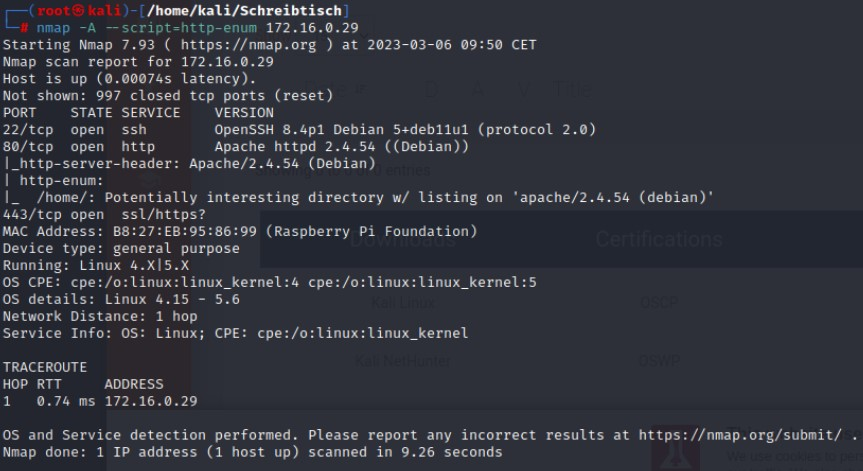
\includegraphics[width = 0.73\textwidth]{http_vulnerbility.jpg}
    \newline
    The script was able to access the ''/home'' path where the apache server has its directories saved. In this case no sensitive files were found. 
    \\&
    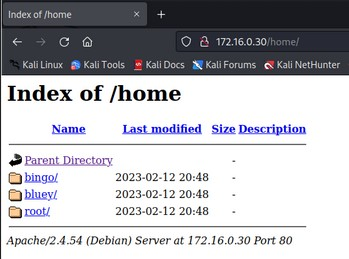
\includegraphics[width = 0.5\textwidth]{dateisystem.jpg} \\
    Recommendation&\\
    \end{tabular*}
    \end{table}

\begin{table}[htb]
    \renewcommand{\arraystretch}{1.5}
    \begin{tabular*}{\textwidth}{|>{\columncolor{red!30}}p{3cm}|p{17.3cm}|}
    \textbf{\large Finding} &\textbf{\large Weak Password for User ''Bluey''} \section*{}\addcontentsline{toc}{section}{Finding 2 - Weak Password for User ''Bluey''}\\
    Risk& Critical\\
    Category&Access Controls\\
    Impact& An attacker can login as the user ''bluey'' and access \ac{ssh}.\\\\ 
    Description& After finding out the user names in the last finding the tool hydra was used to try to brute force the passwords of the users. Therefore we used the following script: \newline hydra -l bluey -P rockyou.txt 172.16.0.29 ssh -t 4 -V -I 
	\newline
	The file "rockyou.txt" provided by kali linux includes a list of popular passwords. The hydra script tries to establish a SSH connection by trying every single one of the passwords. With the option ''-t 4'' four passwords are used at once.
	\newline
	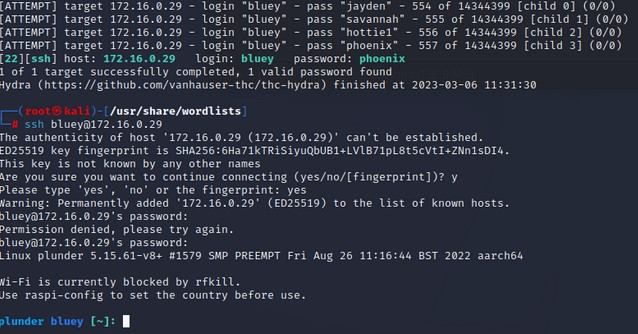
\includegraphics[width = 0.73\textwidth]{brute-force.jpg} 
	\newline
	As shown in the graphic above, Hydra was able to find out the password of the user ''bluey'' which is ''phoenix''. With this information it was possible to establish a SSH connection with the user ''bluey''.
	\\ 
	&\\
    &\\
    Recommendation& Immediate change password of user ''bluey'' and establish an appropriate password policy. 
    \\\\\\\\\\\\\\\\\\\\\\\\\\\\\\  
    \end{tabular*}
    \end{table}

\chapter*{Findings}
\begin{table}[htb]
    \renewcommand{\arraystretch}{1.5}
    \begin{tabular*}{\textwidth}{|>{\columncolor{orange!15}}p{3cm}|p{17.1cm}|}
    \textbf{Finding} & \textbf{No SSH Brute-Force Protection}\\
    Risk& Medium\\
    Category& Misconfiguration\\
    Impact& An attacker is able to brute force the passwords of the ssh user accounts.\\ 
    Description&
    Considering there are no limitations for login attempts are configured performing an brute force attack via the hydra tool is possible (See Finding Weak Password for User ''Bluey'').  
	\\ 
    Recommendation& Limit the login attempts of the users.\\
    &\\
	&\\
	&\\
	&\\
	&\\
	&\\
	&\\
	&\\
    &\\
	&\\
	&\\
	&\\
	&\\
	&\\
	&\\
	&\\ 
    &\\    
	&\\       
    &\\    
    &\\    
	&\\    
	&\\        
    \end{tabular*}
    \end{table}

\section{Finding 4 - SSH Root Access via less}
\hrule
\begin{table}[htb]
    \renewcommand{\arraystretch}{1.5}
    \begin{tabular*}{\textwidth}{|>{\columncolor{red!30}}p{3cm}|p{17.2cm}|}
    \textbf{Finding} & \textbf{SSH Root Access}\\
    Risk& Critical\\
    Category& Access Controls, Privilege Escalation\\
    Impact& An attacker is able to gain SSH root access.\\ 
    Description& After logging into the user account ''bluey'' the command ''sudo -l'' illustrates the users privileges. 
    \newline
    \newline
    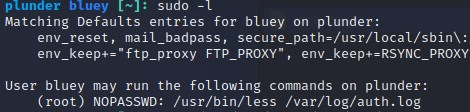
\includegraphics[width=0.73\textwidth]{sudo_l.jpg}
    \newline
    The command disclosed that ''bluey'' has root access for the command: ''/usr/bin/less /var/log/auth.log'' without as password. Although there was initially a misinterpretation of the output when attempting to run ''sudo less'' on a file or accessing the ''auth.log'' file, the command ultimately worked. Upon conducting research on methods for escalating privileges, it was discovered that it is possible to input ''! /bin/bash'' into the less command line, which will grant root access to the bash.
    \newline
    \newline
    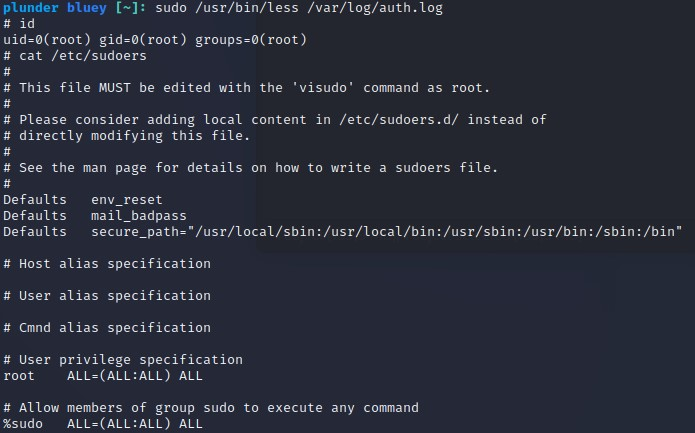
\includegraphics[width=0.73\textwidth]{root_access.jpg}
    \newline
    Executing the command ''id'' will display the current user. The graphic above illustrates that the current user has a uid of zero, which corresponds to the root user.
    The root user has all privileges as shown under the headline ''privilege specification''.
    \\
    \end{tabular*}
    \end{table}
    
\newpage
\begin{table}[htb]
    \renewcommand{\arraystretch}{1.5}
    \begin{tabular*}{\textwidth}{|>{\columncolor{red!30}}p{3cm}|p{17.2cm}|}
    \textbf{Finding} & \textbf{SSH Root Access via less}\\
    
	&\\

    Recommendation& Edit the 'sudoers' file via 'visudo' and delete the last line.\\    
    \end{tabular*}
    \end{table}

\section{Finding 4 - SSH Root Access via less}
\hrule
\begin{table}[htb]
    \renewcommand{\arraystretch}{1.5}
    \begin{tabular*}{\textwidth}{|>{\columncolor{red!15}}p{3cm}|p{17.2cm}|}
    \textbf{Finding} & \textbf{SSH Root Access}\\
    
	&\\

    Recommendation&\\    
    \end{tabular*}
    \end{table}

\chapter*{Findings}
\begin{table}[htb]
    \renewcommand{\arraystretch}{1.5}
    \begin{tabular*}{\textwidth}{|>{\columncolor{red!15}}p{3cm}|p{17.1cm}|}
    \textbf{Finding} & \textbf{SSLv2, SSLv3,TLS 1.1 support}\\
    Risk& High\\
    Category & Misconfiguration\\
    Impact& Decrypt Data, Man in the Middle Attacks \\ 
    Description& The \ac{tls} configuration supports the deprecated protocols: SSLv2, SSLv3, TLS 1.1. Executing the command: ''openssl s\_client --connect 172.16.0.29:433 -ssl2'' opens an SSLv2 connection to the server 172.16.0.29 on port 433 and displays the encryption and certificate information.
    \newline
    \newline
    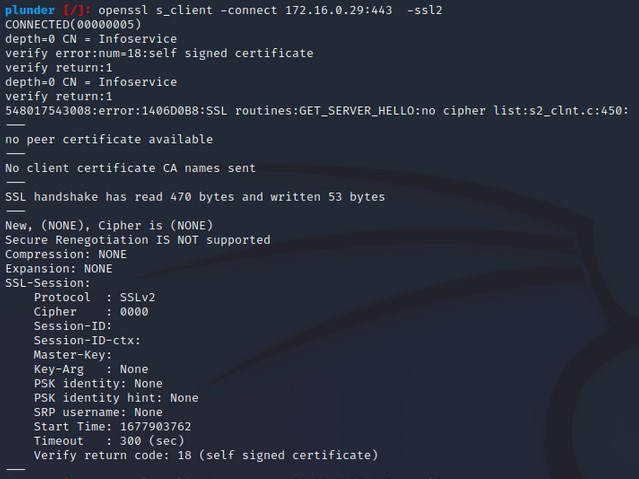
\includegraphics[width=0.73\textwidth]{ssl_2_support.jpg}
    \newline
	\\ 
    Recommendation&\\    
    \end{tabular*}
    \end{table}

\begin{table}[htb]
    \renewcommand{\arraystretch}{1.5}
    \begin{tabular*}{\textwidth}{|>{\columncolor{orange!15}}p{3cm}|p{17.3cm}|}
    \textbf{\large Finding} & \textbf{\large Vulnerable OpenSSH Version}\section*{}\addcontentsline{toc}{section}{Finding 6 - Vulnerable OpenSSH Version}
    \\
    Risk& Medium\\
    Category& Vulnerable Software Version\\
    Impact& An attacker who can access the socket of the forwarding agent remotely may be able to execute unauthorized code with the same privileges as the process or cause a \ac{DoS} situation. An Attacker can perform privilege escalation when AuthorizedKeysCommand/AuthorizedPrincipalsCommand are configured.
    CVE-2021-28041, CVE-2021-41617\\\\ 
    Description&
    An nmap scan illustrated the openssh version. 
    \newline
    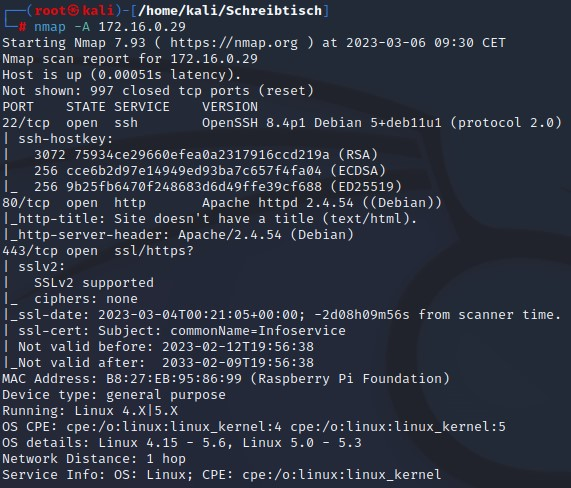
\includegraphics[width=0.73\textwidth]{vulnerable_software.jpg} 
    \newline  
    The openssh version ''OpenSSH 8.4p1 Debian 5+deb11u1 (protocol 2.0)'' has several vulnerabilites under certain circumstances mentioned in the impact part.
	\\ 
	&\\
	&\\ 
    &\\ 
    Recommendation& Patch your OpenSSH Version to a newer, not vulnerable version.\\
    \\\\\\\\\\\\\\\\\\
    \end{tabular*}
    \end{table}



\begin{table}[htb]
    \renewcommand{\arraystretch}{1.5}
    \begin{tabular*}{\textwidth}{|>{\columncolor{orange!15}}p{3cm}|p{17.3cm}|}
    \textbf{\large Finding} & \textbf{\large Vulnerable Apache Version}\section*{}\addcontentsline{toc}{section}{Finding 7 - Vulnerable Apache Version}
    \\
    Risk& Medium\\
    Category& Vulnerable Software Version\\
    Impact& The client may not interpret security-related headers if a malicious backend causes the response headers to be truncated early, resulting in some headers being included in the response body. An attacker can perform HTTP Request Smuggeling due to inconsistend interpretation of HTTP Requests.
    CVE-2022-37436, CVE-2022-36760\\\\ 
    Description&
    An nmap scan illustrated the Apache version. 
    \newline
    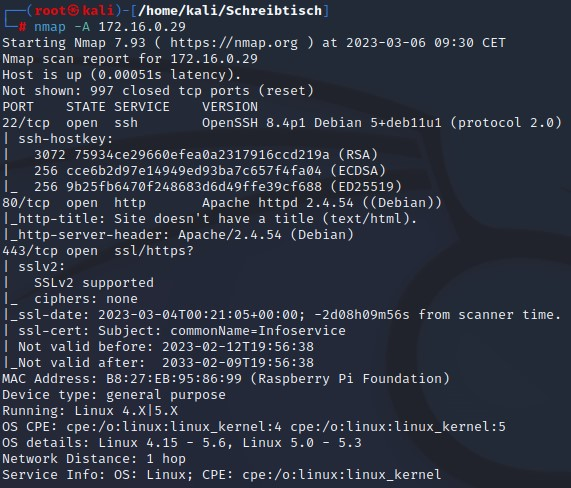
\includegraphics[width=0.73\textwidth]{vulnerable_software.jpg} 
    \newline  
    The apache version ''Apache 2.4.54'' has several vulnerabilites.
	\\ 
	&\\
	&\\
	&\\
    Recommendation& Patch your OpenSSH Version to a newer, not vulnerable version.\\    
    \\\\\\\\\\\\\\\\\\\\\\\\
    \end{tabular*}
    \end{table}

\section{Finding 7 - Root read access on port 433}
\hrule
\begin{table}[htb]
    \renewcommand{\arraystretch}{1.5}
    \begin{tabular*}{\textwidth}{|>{\columncolor{red!15}}p{3cm}|p{17.2cm}|}
    \textbf{Finding} & \textbf{Root read access on port 433}\\
    Risk& High \\
    Category & Broken Access Control, Misconfiguration\\
    Impact& An attacker read access to all files on the server. This can also happen to regular users by accident.\\ 
    Description& 
    After trying to access the server on port 433 with the url https://172.16.0.29:433 an error message was displayed: \newline \newline
    Error opening ''
    548660451168:error:02001002:system library:fopen:No such file or directory:bss\_file.c:169:fopen('','r') \newline
    548660451168:error:2006D080:BIO routines:BIO\_new\_file:no such file:bss\_file.c:172:
    \newline
    After considering serveral option what the purpose of the \ac{https} service running on port 433 was, it turned out that it represents the file system of the server. It is possible to access serveral files on the server.
    \newline
    \newline
    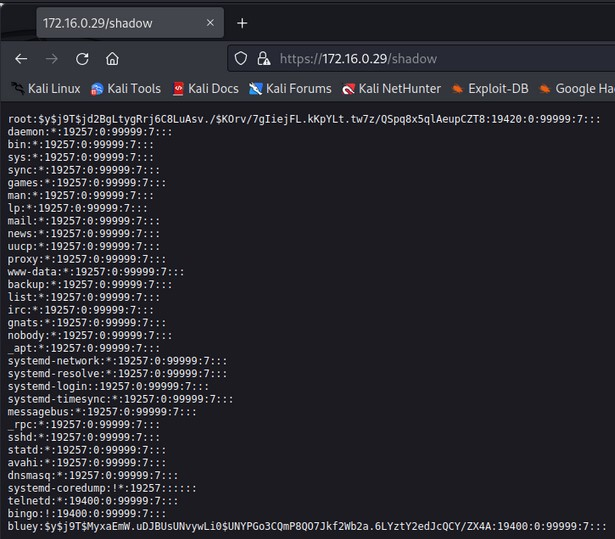
\includegraphics[width=0.73\textwidth]{Webserver_root_access.jpg}
    \newline
    Shown in the graphic above it was possible to access the shadow.txt file of the server where the hashes of all user passwords are listed.
	\\   
    \end{tabular*}
    \end{table}
    \newpage
    \begin{table}[htb]
        \renewcommand{\arraystretch}{1.5}
        \begin{tabular*}{\textwidth}{|>{\columncolor{red!15}}p{3cm}|p{17.2cm}|}
        \textbf{Finding} & \textbf{Root read access on port 433}\\
        
        &\\
    
        Recommendation& Establish correct error handling. To enhance security, it is important to restrict users' access to authorized paths. This can be achieved by prompting for a password when attempting to access the website, or by implementing a login system that requires users to authenticate themselves before accessing the path.\\
        \\\\\\\\\\\\\\\\\\\\\\\\\\\\\\\\\\\\\\\\\\\\\\\\\\\\\\\\\\\\\\\\\\\\  
        \end{tabular*}
        \end{table}

\chapter*{Findings}
\begin{table}[htb]
    \renewcommand{\arraystretch}{1.5}
    \begin{tabular*}{\textwidth}{|>{\columncolor{red!15}}p{3cm}|p{17.1cm}|}
    \textbf{Finding} & \textbf{Root read access on port 433}\\
    
	&\\

    Recommendation&\\    
    \end{tabular*}
    \end{table}


\clearpage
\restoregeometry
}

\chapter{Abkürzungsverzeichnis}

\begin{acronym}
    \acro{DUT}[DUT]{Device Under Test}
    \acro{ssl}[SSL]{Secure Socket Layer}
    \acro{ssh}[SSH]{Secure Shell}
    \acro{http}[HTTP]{Hypertext Transfer Protokoll}
    \acro{tls}[TLS]{Tansport Layer Security}
    \acro{DoS}[DoS]{Denial of Service}
    \acro{https}[HTTPS]{Hypertext Transfer Protokoll Secure}
    \acro{SD}[SD]{Secure Digital}
\end{acronym}

% Beendet eine Seite und erzwingt auf den nachfolgenden Seiten die Ausgabe aller Gleitobjekte (z.B. Abbildungen), die bislang definiert, aber noch nicht ausgegeben wurden. Dieser Befehl fügt, falls nötig, eine leere Seite ein, sodaß die nächste Seite nach den Gleitobjekten eine ungerade Seitennummer hat. 
\cleardoubleoddpage

% pagestyle für gesamtes Dokument aktivieren
\pagestyle{fancy}

%Literaturverzeichnis
\bibliographystyle{unsrtdin}
\bibliography{Literatur}

\end{document}
